\documentclass[11pt]{memoir}

\usepackage{importationsprojet}

\pagestyle{empty}
\setlength{\parindent}{0pt}

\usepackage{ifthen}
\usepackage{multicol}
\usepackage{enumitem}
\usepackage{graphicx}
\usepackage{wrapfig}

\usetikzlibrary{calc}

\newgeometry{margin=1.5cm}

\begin{document}
\begin{questions}

\exercice 

\question Construire un schéma à main levée des deux figures décrites ci-dessous.
\vspace{1em}

\begin{tabular}{cc}\hline
Figure 1 : & Figure 2 : \\\hline
\begin{minipage}{0.4\linewidth}
\begin{itemize}
    \item $A$, $B$ et $C$ sont trois points alignés
    \item $(AB) \perp (BD)$
    \item $BC = \qty{3}{cm}$
\end{itemize}
\end{minipage}
&
\begin{minipage}{0.4\linewidth}
\begin{itemize}
    \item $XY = YZ = \qty{3}{cm}$
    \item $XZ = \qty{5}{cm}$
    \item $WZ = \qty{3}{cm}$ et $(WY) \perp (XZ)$
\end{itemize}
\end{minipage}\\\hline
\end{tabular}

\vspace{1em}

\question Que dire de la nature du triangle $ABD$ ? et du triangle $BCD$ ?
\question Que dire de la nature du triangle $XYZ$ ? et du quadrilatère $WXYZ$ ?

\exercice 

\begin{wrapfigure}{R}{0.15\textwidth}
    \vspace{-1cm}
    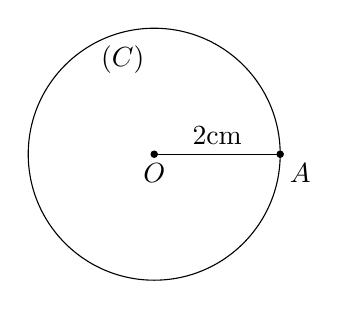
\begin{tikzpicture}[scale=0.8]
        \draw (0,0) circle (2);
        \draw[fill=black] (0,0) circle (0.05);
        \node[below] at (0,0) {$O$};
        \node[below right] at (2,0) {$A$};
        \draw[fill=black] (2,0) circle (0.05);
        \draw (0,0) -- (2,0);
        \node[above] at (1,0) {\qty{2}{cm}}; 
        \node at (-0.5,1.5) {$(\curs{C})$};
    \end{tikzpicture}
\end{wrapfigure}

\question Dans le cercle ci-dessus, quel nom particulier donne-t-on au segment $[OA]$ ?
\question Calculer le périmètre du cercle $(\curs{C})$.
\question Placer un point $B$ sur le cercle $(\curs{C})$. \\De quelle nature est le triangle OAB ?

\exercice

Un train part à 9h30 à Lille et arrive à 10h45 à Paris.
\medskip

\question Combien de temps a duré le trajet ?
\question Convertir le résultat de la question précédente en secondes.
\medskip

Au retour, le train part de Paris à 19h00 et fait une escale à 19h50 à Amiens, puis repart à 20h20 et arrive à Lille à 20h50.
\medskip

\question Combien de temps a duré le trajet Paris-Lille ?
\question Combien de temps a-t-on passé à Amiens en escale ?

\exercice 

Trace le chemin pour aller de \num{12,5} à \num{1} en suivant la règle : on peut monter vers une brique qui contient un nombre plus grand ou descendre vers une brique qui contient un nombre plus petit et on ne peut pas se déplacer à l'horizontale.
\medskip

\begin{center}
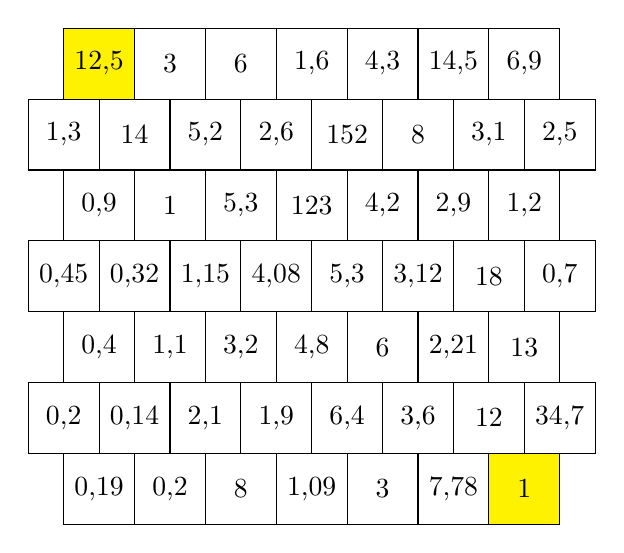
\begin{tikzpicture}[scale=0.9]
    \draw[fill=yellow] (0,0) rectangle (1,-1);
    \draw[fill=yellow] (6,-6) rectangle (7,-7);
    
    \foreach \x in {0,...,7}
    {
        \foreach \y in {0,-2,...,-6} 
        {
            \ifnum\x<7
            \draw (\x,\y) rectangle (\x+1,\y-1);
            \fi
        }
        \foreach \y in {-1,-3,-5}
        {
            \draw (\x-0.5,\y) rectangle (\x+0.5,\y-1);
        }
    }

    \node at (0.5,-0.5) {12,5};
    \node at (1.5,-0.5) {3};
    \node at (2.5,-0.5) {6};
    \node at (3.5,-0.5) {1,6};
    \node at (4.5,-0.5) {4,3};
    \node at (5.5,-0.5) {14,5};
    \node at (6.5,-0.5) {6,9};
    
    \node at (0,-1.5) {1,3};
    \node at (1,-1.5) {14};
    \node at (2,-1.5) {5,2};
    \node at (3,-1.5) {2,6};
    \node at (4,-1.5) {152};
    \node at (5,-1.5) {8};
    \node at (6,-1.5) {3,1};
    \node at (7,-1.5) {2,5};
    
    \node at (0.5,-2.5) {0,9};
    \node at (1.5,-2.5) {1};
    \node at (2.5,-2.5) {5,3};
    \node at (3.5,-2.5) {123};
    \node at (4.5,-2.5) {4,2};
    \node at (5.5,-2.5) {2,9};
    \node at (6.5,-2.5) {1,2};
    
    \node at (0,-3.5) {0,45};
    \node at (1,-3.5) {0,32};
    \node at (2,-3.5) {1,15};
    \node at (3,-3.5) {4,08};
    \node at (4,-3.5) {5,3};
    \node at (5,-3.5) {3,12};
    \node at (6,-3.5) {18};
    \node at (7,-3.5) {0,7};
    
    \node at (0.5,-4.5) {0,4};
    \node at (1.5,-4.5) {1,1};
    \node at (2.5,-4.5) {3,2};
    \node at (3.5,-4.5) {4,8};
    \node at (4.5,-4.5) {6};
    \node at (5.5,-4.5) {2,21};
    \node at (6.5,-4.5) {13};
    
    \node at (0,-5.5) {0,2};
    \node at (1,-5.5) {0,14};
    \node at (2,-5.5) {2,1};
    \node at (3,-5.5) {1,9};
    \node at (4,-5.5) {6,4};
    \node at (5,-5.5) {3,6};
    \node at (6,-5.5) {12};
    \node at (7,-5.5) {34,7};
    
    \node at (0.5,-6.5) {0,19};
    \node at (1.5,-6.5) {0,2};
    \node at (2.5,-6.5) {8};
    \node at (3.5,-6.5) {1,09};
    \node at (4.5,-6.5) {3};
    \node at (5.5,-6.5) {7,78};
    \node at (6.5,-6.5) {1};
    
\end{tikzpicture}
\end{center}


\end{questions}
\end{document}


